\documentclass[letterpaper,twocolumn,10pt]{article}
\usepackage{epsfig,xspace,url}
\usepackage{authblk}
\usepackage{graphicx}
\usepackage{listings}
\graphicspath{ {images/} }

%Your  report  must  be  3  pages  long.  You  must  use  a  two-‐‐column  format,  10-‐‐pointtimes  new  roman  font,  and  your  lines/paragraphs  must  be  single-‐‐spaced.  Your report must not include any code. However, you must make your code available on a web page or a repository and provide the pointer to that page in your report.

\title{Third Party Encrypted Storage}
\author{Travis Taylor, John Robe, and Daniel James}
\affil{School of Computing, University of Utah}

\begin{document}

%Code listing formatting
\lstdefinestyle{codestyle}{
    basicstyle=\footnotesize,
    frame=single,
    breaklines=true
}
\lstset{style=codestyle}


\maketitle

%Introduction  –  Motivate  and  introduce  the  problem  you  are  solving.  Very briefly summarize your methodology, your experiments, and your important results.
\section{Introduction}

Remembering a good password is hard. Unsurprisingly most people take the path of least resistance, and simply don't use good passwords. Frequently user passwords consist of personal information or absolutely simple ones to guess like \textit{1234}\cite{easypass}. Many organizations require that you use certain combinations of letters, numbers, and symbols. This frequently annoys users, as it makes passwords more difficult to use. Given this constraint on passwords, many users make one password that will satisfy many of the complexity requirements for most passwords, and simply use that everywhere. This is possibly worse than a simple password, as once one of those are compromised, and this happens with somewhat alarming frequency\cite{databreach}, the attacker has access to all of your other accounts. Even the most secure password policies are vulnerable against social engineering and phishing. A recent survey determined that 42\% of IT decision makers listed phishing as one of their top three security concerns\cite{phishing}. Training employees to avoid phishing attacks is also expensive and not 100\% effective.

There are a few current solutions to this. One of the most common allows you to log in to services using an API provided by many commonly used services like Facebook, Google, and Twitter. This requires integration on the services part to use the third party API. This presents a new problem, now those third-party services have all your information about what services you use, as well as holding a lot of Personal Identifiable information (PII). Many users don't like the idea of these third-party services having so much personal information about them, and thus don't even use them, or don't want to use them to log into other services.

Thus, we chose to not use passwords at all, at least, not in the traditional sense. We chose to implement a system in which a third party service holds information that would usually be guarded by a user password. This third party service would work with any application that desires to get information, such as a strong password or simply an email, from the user. The user just has to store this cryptographically strong key on their device, and allow access by accepting on a portal application. The portal application unlocks the data on the server temporally, and sends it to the requesting application.  We show that this is feasible with our implementation and removes the need for traditional passwords. 

%Related work – Summarize the existing work related to your problem.
\section{Related Work}
	Two factor authentication has been a common solution to user authentication, only gaining more popularity over the past few years; in fact it has recently become a requirement for employees at the University of Utah. Our solution is very similar to 2FA, except it is getting rid of the password step altogether. Other solutions to the password problem is to assign \cite["Smart Cards"]{card} to the user, and use those to assign passwords for users. Our solution uses common user devices (cell phones) instead of expensive proprietary cards. 

%Adversary model – Describe the adversary you are securing against.
\section{Adversary Model}
    We look at our problem from multiple attack vectors:
    \begin{itemize}
    \item \textit{Attacker with copy of database} - This is the most basic case, if an adversary gains a copy of the database via some means.
    \item \textit{Government/Authority} - This is the case where a government or authority subpoenas the database from the authentication server. This subtly different from the first case, as the owner of the database is coerced to provide any keying information to that authority.
    \item \textit{MITM\footnote{Man in the middle; the act of impersonating the server}/Impersonation} - The case where an entity stands in between the user and the server, having the ability to manipulate messages going both ways.
    \item \textit{Phishing} - Tricking a user into revealing their password.
    \end{itemize}

%Methodology – Describe your solution and any other methods you have used to solve your problem.
\section{Design}

Our solution to this problem is to not use passwords at all. Instead of remembering passwords, a user's device (such as a smartphone) remembers it for him. Since a computer doesn't have the memory limitations a human does, it can have absolutely random passwords of sufficiently large length. 

Our basic design consists of four entities; see Figure \ref{design}.
\begin{itemize}
    \item \textbf{User} - The user that desires to use our application, to store their data securely
    \item \textbf{Authentication Server} - The server that will store the encrypted data for the user, without having the key.
    \item \textbf{Portal Application} - This is the application that retrieves data from the user to unlock the data on the authentication server.
    \item \textbf{Demo Application} - This application is the entity that requests data about the user.
\end{itemize}

\begin{figure*}[ht]
\centering
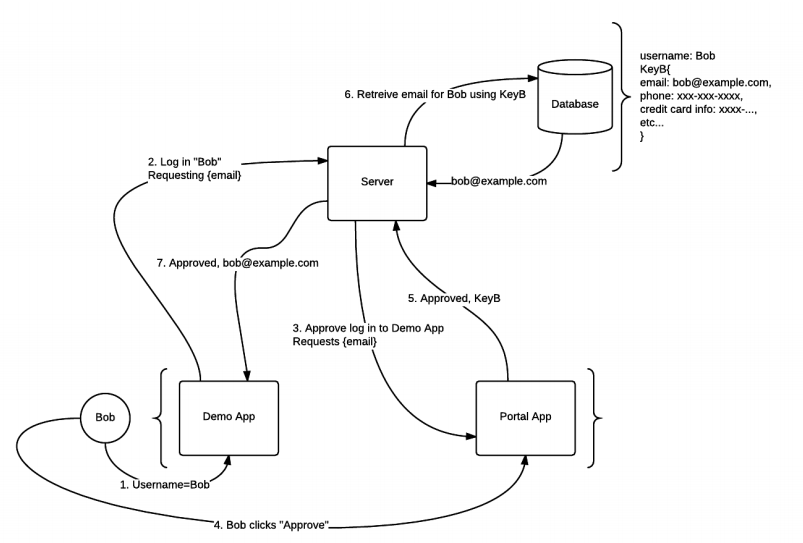
\includegraphics[width=\textwidth]{Design}
\caption{Overall system design}
\label{design}
\end{figure*}

We chose to split the Authentication server and the Portal application to mitigate risk in the event of a database breach. In the case where the database was compromised, the attacker would still not have the key required to decrypt any of the data. The Portal application will store the key. The portal application may be further protected by the device it is installed on, such as the PIN required to unlock a smartphone. Once the authentication server uses the key, the authentication server forgets the key.

%TODO Perhaps had more design choices?

An example of a successful authentication is shown in Figure \ref{messageflow}. You can see here that from our user, Bob's, perspective that he only has to answer a permission question, and the most of the burden is taken care for him outside of his view.

\begin{figure}[ht]
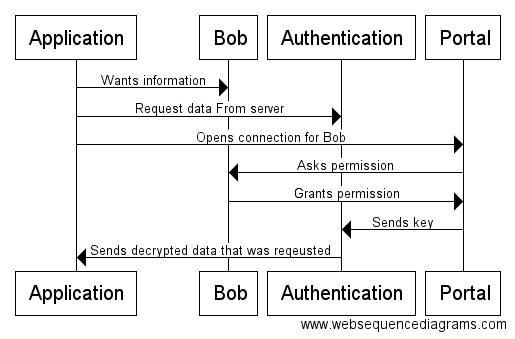
\includegraphics[width=0.45\textwidth]{messageDiagram}
\caption{Message Flow}
\label{messageflow}
\end{figure}

%Describe  your  experiments  and  your results. Discuss your results.
\section{Implemention}

\paragraph{RPCs and Message Formats}
    We chose to use Thrift\cite{thrift} as our RPC\footnote{remote procedure call} and message formatting framework. We chose this primarily because it allows for multiple different output languages from it's initial IDL\footnote{interface definition language}. The way Thrift works is you define a set of structures and functions in an IDL, and then compile it to the various langauges you wish to use it in. 
    
%A snippet of our Thrift IDL file:

%\begin{figure}[h]
%\begin{minipage}{\linewidth}
%\lstinputlisting[firstline=0,lastline=22]{../thrift/cs5490.thrift}
%\caption{Example Thrift File}
%\label{ref:code}
%\end{minipage}
%\end{figure}

\subsection{Authentication Server}
    The authentication server deals with holding the encrypted data. It is relatively simple, as it merely has to hold a 2 column table, and provide the ability to decrypt with a given key. The server provides this functionality through Apache Thrift\cite{thrift}. It provides some simple functions:
    \begin{itemize}
        \item \textbf{createAccount} - Creates the account for the user, and generates the key for it.
        \item \textbf{requestPermission} - The application requesting access will call this function with the requested data fields and user.
        \item \textbf{checkForPermissionRequest} - Portal can check if it has any pending requests\footnote{In lieu of push notifications, we moved for polling due to time constraints} 
        \item \textbf{decideRequest} - Once the user decides what they want to do, the portal application will call this with the decision and, if in the affirmative, the key.
        \item \textbf{checkForPermissionGranted} - The demo application can poll with a request ID to see if their request has been confirmed or denied.
    \end{itemize}

The backend storage is SQLite, given the simple nature of the data. This could have also been done in a key-value pair database, however, that would have required setting up another server for this.

\subsection{Portal and Demo Application}
Both the portal and demo application were written in Java, also using Thrift. However, these were only written for the demonstration of the authentication server. Because of Thrift, it would be possible to easily support many other languages. In order for this scheme to be feasible, the portal app would need to run on many different types of devices. Using Thrift, we could create libraries for many programming languages and encourage developers to implement our authentication scheme into their applications.

The portal application has two functionalities. First it provides a form to the user so that they can register a new account with the authentication server. Once an account is created a key is stored on the device and the portal application enters the background. The portal application notifies the user with a pop up whenever a request is created for the user's account.

The demo application is a simple application that asks for your username. Once authenticated, the application displays the user's information in a table. 


% Summarize  your  work  and  your  results.  Indicated  any  future directions.
\section{Conclusion}
    We have shown that it's not required for a user to remember passwords to obtain the same goal of only allowing authorized parties access to private information. We did this by implementing a system that holds encrypted user data without holding the key itself. This key is stored on the device, as opposed to being generated by a traditional user password. This mitigates many of the threats presented in our adversary model. In the most simple case, however the adversary obtains the database, its still encrypted. The database, assuming it was correctly programmed, will only have the key for a short period of time, before it dumps it from memory. There is simply no encryption key for the attacker to get, unless they impersonated the authentication server. This case itself is mitigated by the fact that we require SSL on all links.

\subsection{Alterative Methods}

What we have done is essentially shift the problem from \textit{what you know} to \textit{what you have} \cite[Chapter~9]{privcomm}. This method has its own unique set of problems. What if the user loses their device? They are suddenly without access to their information, so some kind of \textit{what you know} approach would seem to be required here as well, if only to recover the data in the case of a lost device.

It's also possible to shift the decryption of the data away from the server. Instead of having the server decrypt the data, it could act as dumb data storage and instead forward encrypted data to the clients device. The client device could then decrypt it locally and send it to the application that requested it. In this way, you are really just storing your encrypted data \textit{in the cloud}, and retrieving it from one or more devices. 

%Talk about how we could have done a few things differently, like having the portal generate the key and then send it to the server, as this would have allowed it to generate it from a password and not have to even talk to the server.


%List all the references you have used for this work.
{
    \small
    \bibliographystyle{acm}
    \bibliography{biblio}
}

\end{document}
